\section{Cross-Forest trust Attack}


\subsection{Cross-Forest Kerberoasting}

Kerberos attacks such as Kerberoasting and ASREPRoasting can be performed
across trusts, depending on the trust direction. In a domain with either an
inbound or bidirectional domain/forest trust, various attacks to gain a
foothold. Sometimes privilege scalation is not possible in the current domain,
but instead it is possible to obtain a Kerberos ticket and crack a hash for an
administrative user in another domain that has Domain/Enterprise Admin
privileges in both domains.

\subsubsection{Windows}
use of the \verb+-SPN+ and \verb+-Domain+ set to the trusting domain on \verb+Get-DomainUser+~\ref{tool:powerview:enum} Then a kerberoast~\ref{kerberos:kerberoasting} can be performed on the trusted domain.

\subsubsection{Linux}
From time to time, see users or admins from one domain as members of a group in another domain. Since only i\emph{Domain Local Groups} allow users from outside their forest, it is not uncommon to see a highly privileged user from Domain A as a member of the built-in administrators group in domain B when dealing with a bidirectional forest trust relationship.

To enumerate \verb+GeUserSPNs+~\ref{tool:impacket:GetUserSPNs} with
credentials for a user that can authenticate into the other domain and specify
the \verb+-target-domain+. the flag \verb+-request+ (plus \verb+-outputfile+)
provide the TGS.

\subsection{Admin Password Re-Use  and Group Membership}
In a situation of a  bidirectional forest trust managed by admins from the same
company. When the Domain A is controlled and a cleartext passwords or NT hashes
for either the built-in Administrator account or an account that is part of the
Enterprise Admins or Domain Admins group in Domain A is available and Domain B
has a highly privileged account with the same name. It is worth checking for
password reuse across the two forests in this situation. 

For example, Domain A would have a user named \verb+adm_bob.smith+ in the
Domain Admins group, and Domain B had a user named \verb+bsmith_admin+.
Sometimes, the user would be using the same password in the two domains, and
owning Domain A instantly gave me full admin rights to Domain B.

Somtimes users or admins from Domain A as members of a group in Domain B. Only
\emph{Domain Local Groups} allow security principals from outside its forest.
Somtimes a Domain Admin or Enterprise Admin from Domain A as a member of the
built-in Administrators group in Domain B in a bidirectional forest trust
relationship. Taking over this admin user in Domain A, we would gain full administrative access to Domain B based on group membership.

\verb+Get-DomainForeignGroupMember+~\ref{tool:powerview:enum} allow to
enumerate groups with users that do not belong to the domain, also known as
foreign group membership. 


\subsection{Cross Forest SID History Abuse}

SID History can also be abused across a forest trust. If a user is migrated
from one forest to another and SID Filtering is not enabled, it becomes
possible to add a SID from the other forest, and this SID will be added to the
user's token when authenticating across the trust. If the SID of an account
with administrative privileges in Forest A is added to the SID history
attribute of an account in Forest B, assuming they can authenticate across the
forest, then this account will have administrative privileges when accessing
resources in the partner forest.

\begin{figure}[!ht]
  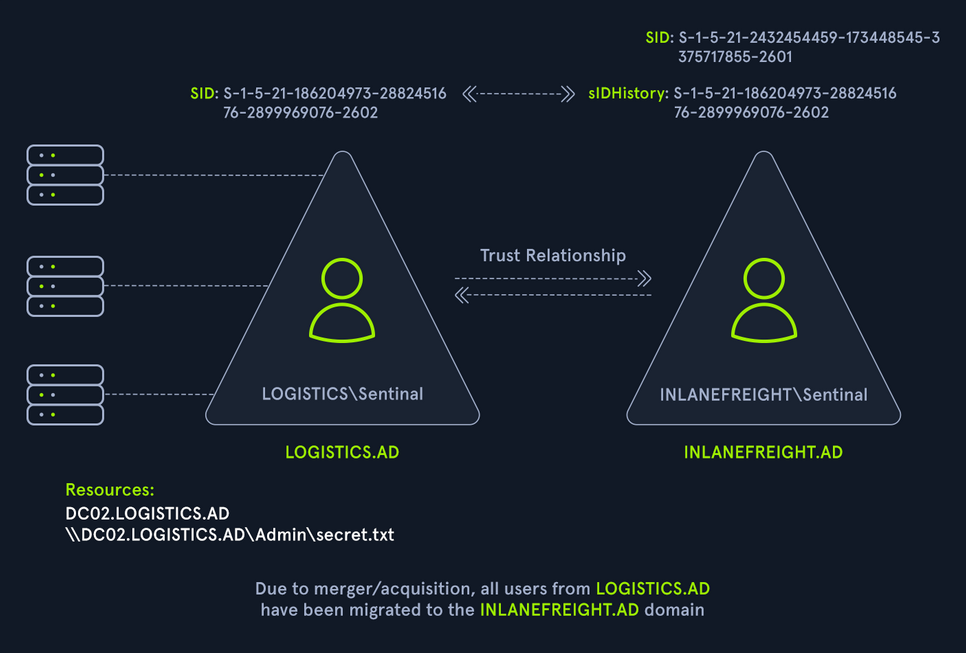
\includegraphics[width=\linewidth]{ad/trust/images/cross-forest-sid-history.png}
  \caption{Cross forest AD trust SIDHistory}
  \label{fig:cross-forest-sid-history}
\end{figure}

In the previous diagram, \verb+jjones+ user being migrated
from the \verb+INLANEFREIGHT.LOCAL+ domain to the \verb+CORP.LOCAL+ domain in a different
forest. If SID filtering is not enabled when this migration is made and the
user has administrative privileges (or any type of interesting rights such as
ACE entries, access to shares, etc.) in the \verb+INLANEFREIGHT.LOCAL+ domain,
then they will retain their administrative rights/access in
\verb+INLANEFREIGHT.LOCAL+ while being a member of the new domain,
\verb+CORP.LOCAL+ in the second forest.



